\documentclass[11pt,]{article}
\usepackage[left=1in,top=1in,right=1in,bottom=1in]{geometry}
\newcommand*{\authorfont}{\fontfamily{phv}\selectfont}
\usepackage[]{mathpazo}


  \usepackage[T1]{fontenc}
  \usepackage[utf8]{inputenc}




\usepackage{abstract}
\renewcommand{\abstractname}{}    % clear the title
\renewcommand{\absnamepos}{empty} % originally center

\renewenvironment{abstract}
 {{%
    \setlength{\leftmargin}{0mm}
    \setlength{\rightmargin}{\leftmargin}%
  }%
  \relax}
 {\endlist}

\makeatletter
\def\@maketitle{%
  \newpage
%  \null
%  \vskip 2em%
%  \begin{center}%
  \let \footnote \thanks
    {\fontsize{18}{20}\selectfont\raggedright  \setlength{\parindent}{0pt} \@title \par}%
}
%\fi
\makeatother




\setcounter{secnumdepth}{0}


\usepackage{graphicx,grffile}
\makeatletter
\def\maxwidth{\ifdim\Gin@nat@width>\linewidth\linewidth\else\Gin@nat@width\fi}
\def\maxheight{\ifdim\Gin@nat@height>\textheight\textheight\else\Gin@nat@height\fi}
\makeatother
% Scale images if necessary, so that they will not overflow the page
% margins by default, and it is still possible to overwrite the defaults
% using explicit options in \includegraphics[width, height, ...]{}
\setkeys{Gin}{width=\maxwidth,height=\maxheight,keepaspectratio}


\title{Leveraging the `Black Box': Random Forest Adjustment for Causal Inference  }



\author{\Large Miles D. Williams\vspace{0.05in} \newline\normalsize\emph{University of Illinois at Urbana-Champaign}  }


\date{}

\usepackage{titlesec}

\titleformat*{\section}{\Large\bfseries}
\titleformat*{\subsection}{\large\itshape\bfseries}
\titleformat*{\subsubsection}{\normalsize\itshape}
\titleformat*{\paragraph}{\normalsize\itshape}
\titleformat*{\subparagraph}{\normalsize\itshape}


\usepackage{natbib}
\bibliographystyle{plainnat}
\usepackage[strings]{underscore} % protect underscores in most circumstances



\newtheorem{hypothesis}{Hypothesis}
\usepackage{setspace}


% set default figure placement to htbp
\makeatletter
\def\fps@figure{htbp}
\makeatother

\usepackage{amsmath}
\usepackage{dcolumn}

% move the hyperref stuff down here, after header-includes, to allow for - \usepackage{hyperref}

\makeatletter
\@ifpackageloaded{hyperref}{}{%
\ifxetex
  \PassOptionsToPackage{hyphens}{url}\usepackage[setpagesize=false, % page size defined by xetex
              unicode=false, % unicode breaks when used with xetex
              xetex]{hyperref}
\else
  \PassOptionsToPackage{hyphens}{url}\usepackage[draft,unicode=true]{hyperref}
\fi
}

\@ifpackageloaded{color}{
    \PassOptionsToPackage{usenames,dvipsnames}{color}
}{%
    \usepackage[usenames,dvipsnames]{color}
}
\makeatother
\hypersetup{breaklinks=true,
            bookmarks=true,
            pdfauthor={Miles D. Williams (University of Illinois at Urbana-Champaign)},
             pdfkeywords = {},  
            pdftitle={Leveraging the `Black Box': Random Forest Adjustment for Causal Inference},
            colorlinks=true,
            citecolor=blue,
            urlcolor=blue,
            linkcolor=magenta,
            pdfborder={0 0 0}}
\urlstyle{same}  % don't use monospace font for urls

% Add an option for endnotes. -----


% add tightlist ----------
\providecommand{\tightlist}{%
\setlength{\itemsep}{0pt}\setlength{\parskip}{0pt}}

% add some other packages ----------

% \usepackage{multicol}
% This should regulate where figures float
% See: https://tex.stackexchange.com/questions/2275/keeping-tables-figures-close-to-where-they-are-mentioned
\usepackage[section]{placeins}


\begin{document}
	
% \pagenumbering{arabic}% resets `page` counter to 1 
%
% \maketitle

{% \usefont{T1}{pnc}{m}{n}
\setlength{\parindent}{0pt}
\thispagestyle{plain}
{\fontsize{18}{20}\selectfont\raggedright 
\maketitle  % title \par  

}

{
   \vskip 13.5pt\relax \normalsize\fontsize{11}{12} 
\textbf{\authorfont Miles D. Williams} \hskip 15pt \emph{\small University of Illinois at Urbana-Champaign}   

}

}






\vskip -8.5pt


 % removetitleabstract

\noindent \doublespacing 

\hypertarget{introduction}{%
\section{Introduction}\label{introduction}}

Over the past several years, a literature centered on the application of
machine learning techniques to causal identification has grown rapidly.
These efforts have generated promising new aproaches for those eager for
more flexible and robust techniques for recovering causal estimates with
observational data. Among the myriad methods that have been considered,
Random Forest Regression (RF) has become increasingly popular relative
to alternatives. Since its development by Breiman (2001), RF has become
one of the most widely used machine learning predictors in use across a
range of scientific fields---due in no small part to its high level of
predictive performance and simultaneous resistance to overfitting (Wager
2016).

However, RF to-date has been of limited utility for political
scientists. Its predictive performance notwithstanding, RF is a
``black-box,'' scoring low on interpretability---a real handicap in a
discipline that prizes interpretable marginal effects and test
statistics. For this reason, RF is rarely applied by political
scientists, and what applications do appear in the literature are
restricted to exercises in prediction or measurement. Hill and Jones
(2014), for instance, use RF to test the predictive power of various
political, economic, and social conditions for state repression. Bonica
(2018) uses RF to assess the predictive power of campaign contributions
on roll call votes in the U.S. Congress. Meanwhile, Carroll and Kenkel
(2019) use RF, in addition to other machine learning algorithms, to
generate a proxy for relative military power among states.

It would be a misconception, however, to suppose that RF is unusable for
identifying causal relationships. For example, given the nonparametric
approach taken by RF, it comes as little surprise that it has found a
home among those who study the estimation of heterogeneous treatment
effects (e.g., Athey and Imbens 2015; Foster et al.~2011; Su et
al.~2009; Zeileis et al.~2008). These studies are joined by a broader
literature that has developed creative applications of black-box machine
learning techniques to causal inference (for examples see Wager 2016).

These new applications aside, it seems unlikely that political science
will trade its workhorse methods, like linear and generalized linear
regression models and matching, for approaches like RF any time soon.
Not all research questions demand estimation of heterogeneous treatment
effects, and the benefit of learning new machine learning techniques
relative to the costs in time and energy required to become familiar
with them is often perceived as low.

In the face of such hesitancy, I develop a novel application of RF that
leverages the power of its black-box (nonparametric) characteristics,
while permiting estimation of meaningful (and interpretable) marginal
effects. The approach I lay out here, which I call Random Forest
Adjustment (RFA), leverages the simultaneous predictive power, and
resistance to overfitting, of RF to pre-process observational data prior
to estimating an average treatment effect (ATE). The approach proceeds
in three simple steps: (1) compute and collect the residuals of
out-of-bag (OOB) predictions of a RF model fitted using the outcome of
interest as the response and a set of confounding covariates as
predictors; (2) repeat setp 1, but with the causal variable of interest
as the response and the confounding covariates as predictors; (3)
regress the residual variation in the outcome variable on that of the
causal variable and use the estimated coefficient on the treatment
variable residuals as the ATE.

As I will demonstrate, this approach offers a robust (unbiased and
efficient) estimate of the ATE as compared with two well-validated
alternative (and more common) approaches: optimal full matching (using
Mahalanobis Distance), and an interactive multiple regression model, as
proposed by Lin (2013).

However, as I further demonstrate, the improved accuracy in estimated
ATEs generated by RFA comes at the cost of a marginal decline in
generalizability. As Aronow and Samii (2016) highlight, studies that
rely on a relatively comprehensive nominal sample in observational
settings generate causal effects using only a limited effective sample
when accounting for regression weights. OLS, for instance, gives greater
weight to observations not well explained by other covariates included
as predictors in a linear model.

We should not bemoan this feature of RFA and other adjustment
strategies. Having an effective sample composed of comparable
observations is necessary for estimating internally valide causal
estimates. The improved accuracy of RFA necessarily comes at the cost of
a slightly more limited effective sample---a more comprehensive
effective sample would in fact suggest that RFA poorly adjusts for
variation in the data accounted for by confounding covariates.

Even so, limited generalizability notwithstanding, analysis demonstrates
that the diminished overlap between nominal and effective samples
produced by RFA is not overwhelming.

In the following section I offer an overview of the approach. I then
validate it via a series of Monte Carlo simulations, comparing its
performance to other other approaches shown be effective: optimal full
matching, and the interactive multiple regression model specification
suggested by Lin (2013). The results highlight the robustness of RFA to
\emph{complex confounding}---nonlinear and complex functional forms in
the relationship between confounding covariates and a treatment and
response. Further, the analysis reveals greater generalizability of RFA
estimates of treatment effects compared to alternative approaches. As
Aronow and Samii (2016) argue, when researchers use multiple regression
to recover causal estimates with observational data, the effective
sample produced by regression weights is often limited relative to the
nominal sample---the full sample used to estimate the linear regression
model. While RFA similarly relies on a limited effective sample to
recover marginal effects, the RFA effective sample has greater overlap
with the nominal sample than either full matching or multiple
regression. RFA estimates, while still being \emph{local}, generalize to
a broader set of the nominal sample than with other approaches.

I end with an application RFA to a replication of Nielsen et al.~(2011)
who assess the causal effect of foreign aid shocks on the likelihood of
violent armed conflict. RFA estimates differ in important ways from
those identified by the authors. Nielsen et al.~(2011) find that
negative shocks increase the likelihood of conflict, while positive
shocks have no effect. Conversely, while RFA estimates also indicate a
positive effect of negative shocks on the likelihood of conflict, they
identify a significant and negative estimate for the effect of positive
shocks on conflict. The results obtained via RFA square better with
existing theory on the role of power parity on likelihood of war (see
Reed 2003). In addition, assessment of the degree of overlap between the
effective and nominal samples associated with RFA and alternative
estimators supports the greater generalizability of RFA estimates.

\hypertarget{random-forest-adjustment}{%
\section{Random Forest Adjustment}\label{random-forest-adjustment}}

RFA, like other approaches to adjusting for the influence of confounding
covariates, is applicable in settings where one wishes to estimate the
ATE of some intervention or causal variable, but random assignment is in
doubt. That is, one suspects propensity to receive some ``treatment'' to
be dependent on unit characteristics of individual observations. Such is
often the case in observational settings where treatment was not
randomly assigned by a researcher, or else in field experiments where
infelicities in design put random assignment in doubt.

Various strategies for dealing with this problem exist. Matching and its
many permutations are one example, while regression-based approaches
comprise another. However, these approaches, as described above, usually
provide only local average treatment effects (LATEs). As a result, while
being internally valid in many settings, both matching and multiple
regression raise concerns about external validity.

Parametric regression models also pose additional problems. For example,
in a setting with panel data, multiple regression may fail to account
for heterogeneity in the confounding influence of covariates between
clusters. Further, multiple regression may fail to account for
nonlinearities or interactions in the d.g.p. Without perfect knowledge
about the true d.g.p. under investigation, a researcher often does not
know how to specify the ``correct'' model. Consequently, model
mispecification may introduce bias into the estimated causal effect of
interest---even if the research has ``controlled'' for all relevant
confoudning variables.

RFA provides an alternative adjustment strategy for generating an ATE
from observational data. The procedure consists of three steps. It
begins by using the out-of-bag (OOB) prediction for a response (\(y_i\))
and some causal variable of interest (\(z_i\)) as a function of
covariates \(x_{ik} \in X_i\) where
\(y_i,z_i \not\!\perp\!\!\!\perp X_i\). The variables \(y_i\) and
\(z_i\) denote vectors of response and treatment values for the
\(i^\text{th}\) observation where \(i \in I = \{1,2,...,n \}\).

Because \(z_i\) and \(y_i\) are not independent of \(X_i\), the
estimated slope coefficient (\(\alpha_1\)) from the following linear
model estimated via OLS will not reflect the true ATE of \(z_i\) on
\(y_i\): \[y_i = \alpha_0 + \alpha_1z_i + \epsilon_i. \tag{1}\]

RFA's solution to this problem is to partial out the variation in
\(y_i\) and \(z_i\) explained by \(X_i\) prior to estimating the ATE as
follows:

\begin{enumerate}
\def\labelenumi{\arabic{enumi}.}
\tightlist
\item
  First, fit \(y_i\) as a function of \(X_i\) via a RF model and
  estimate the OOB observation-specific residuals:
\end{enumerate}

\[
\begin{aligned}
\hat{y}_i & = \hat{f}(X_i), \\
\hat{y}_i^\varepsilon & = y_i - \hat{y}_i.
\end{aligned} \tag{2}
\]

\begin{enumerate}
\def\labelenumi{\arabic{enumi}.}
\setcounter{enumi}{1}
\tightlist
\item
  This step is then repeated for \(z_i\):
\end{enumerate}

\[
\begin{aligned}
\hat{z}_i & = \hat{g}(X_i), \\
\hat{z}_i^\varepsilon & = z_i - \hat{z}_i.
\end{aligned} \tag{3}
\]

\begin{enumerate}
\def\labelenumi{\arabic{enumi}.}
\setcounter{enumi}{2}
\tightlist
\item
  Finally, the ATE, adjusting for the confounding influence of \(X_i\),
  is obtained by estimating the following linear model via OLS:
\end{enumerate}

\[\hat{y}_i^\varepsilon = \beta_0 + \beta_1\hat{z}_i^\varepsilon + \mu_i.\tag{4}\]

The estimate for \(\beta_1\) in the above denotes the ATE.

One advantage of RFA is that it sidesteps incidental functional form
assumptions that parametric adjustment strategies impose. This can be
seen by considering the following fact about a linear regression model
as estimated with OLS.

With the covariates given in the preceding section, define the matrix
\(\mathbf{W}\) as \[
\mathbf{W} = 
\begin{bmatrix}
1 & z_1 & x_1^1 & \cdots & x_1^k \\
\vdots & \vdots & \vdots & \ddots & \vdots \\
1 & z_n & x_n^1 & \cdots & x_n^k
\end{bmatrix}_{n,k+2}\tag{5}
\] and define the matrix \(\mathbf{y}\) as \[
\mathbf{y} = 
\begin{bmatrix}
y_1 \\
\vdots \\
y_n
\end{bmatrix}_{n,1}.\tag{6}
\] Using OLS, we estimate the linear model
\[\mathbf{y} = \mathbf{W}\boldsymbol{\beta} + \boldsymbol{\epsilon},\]
where the solution for the parameters to be estimated is \[
\hat{\boldsymbol{\beta}} = 
\begin{bmatrix}
\hat{\beta}_0 \\
\hat{\beta}_1 \\
\hat{\beta}_2^1 \\
\vdots \\
\hat{\beta}_{k+2}^k
\end{bmatrix} = (\mathbf{W}^\top\mathbf{W})^{-1} (\mathbf{W}^\top \mathbf{y}).\tag{7}
\] The parameter \(\hat{\beta}_1 \in \hat{\boldsymbol{\beta}}\) is the
estimated effect of \(z_i\) (the causal variable of interest in our
running example).

This approach is potentially problematic for the following reason.
Consider an equivalent way of generating \(\hat{\beta}_1\) via OLS.

\begin{enumerate}
\def\labelenumi{\arabic{enumi}.}
\tightlist
\item
  Estimate a linear model excluding \(z_i\) from the matrix
  \(\mathbf{W}\) and with \(\mathbf{y}\) as the left-hand side variable.
  Denote the new \(n \times k + 1\) matrix that excludes the causal
  variable interest as \(\mathbf{X}\). After estimating this model using
  the same procedure outlined above, generate predicted values of the
  outcome variable and estimate the model residuals (note the similarity
  to step 1 of RFA).
\end{enumerate}

\[
\begin{aligned}
\hat{\mathbf{y}} & = \mathbf{X}\hat{\boldsymbol{\gamma}}, \\
\hat{\mathbf{y}}^\epsilon & = \mathbf{y} -  \hat{\mathbf{y}}.
\end{aligned}\tag{8}
\]

\begin{enumerate}
\def\labelenumi{\arabic{enumi}.}
\setcounter{enumi}{1}
\tightlist
\item
  Repeat the above, but have the \(n \times 1\) matrix \(z\) (a matrix
  of values for the causal variable) be the left-hand side variable
  (again, note the similarity to step 2 of RFA).
\end{enumerate}

\[
\begin{aligned}
\hat{\mathbf{z}} & = \mathbf{X}\hat{\boldsymbol{\delta}}, \\
\hat{\mathbf{z}}^\epsilon & = \mathbf{z} -  \hat{\mathbf{z}}.
\end{aligned}\tag{9}
\]

\begin{enumerate}
\def\labelenumi{\arabic{enumi}.}
\setcounter{enumi}{2}
\tightlist
\item
  Finally, estimate \(\beta_1\) via OLS where the linear model is
  specified as
\end{enumerate}

\[\hat{y}_i^\epsilon = \mu + \beta_1\hat{z}_i^\epsilon + \varepsilon_i.\tag{10}\]

The \(\hat{\beta}_1\) generated from step 3 will be equivalent to the
one estimated above.

At this point, it (hopefully) should be clear why a linear regression
model is potentially problematic. This parametric approach, while
imposing the assumption that \(\hat{y}^\epsilon_i\) and
\(\hat{z}^\epsilon_i\) are linearly related, also imposes the assumption
that the confounding variables are linearly and additively associated
with \(y_i\) and \(z_i\). And this is only the first layer of an onion
of linear additive models within linear additive models which could be
used to estimate equivalent parameters for all of the variables
contained in \(\mathbf{W}\). This is not to mention the googleplex of
potential ``sub''-parameters implied by assuming linearity and
additivity \emph{all the way down}. If in any of the linear additive
models upon linear additive models is misspecified, this portends bias
in \(\hat{\beta}_1\).

This is one place where RFA shines. RFA imposes no functional form on
the relationship between the confounders and the response and causal
variable, and it also imposes no functional form assumptions about how
any and all of the confounders relate to each other. It sidesteps the
Russian doll altogether as it isolates the residual variation in the
response and causal variable.

Of course, other approaches impose minimal functional form assumptions
as well---matching on a distance metric, for example. And the potential
issues with parametric regression-based adjustment notwithstanding, in
many applied settings methods like multiple regression and matching have
strong internal validity. However, as Aronow and Samii (2016)
demonstrate, in providing internally valid causal estimates, both
regression and matching often only provide \emph{local} average
treatment effects. Drawing a distinction between ``nominal'' and
``effective'' samples, Aronow and Samii (2016) point out that multiple
regression differentially weights observations included in a nominal
sample (the total set of cases a researcher may wish to generalize to),
generating estimates for a causal variable of interest that only apply
to a smaller effective sample (based on which observations receive
greatest weight by multiple regression). As they show, the effective
sample can differ markedly from the nominal sample, which restricts the
generalizability of causal estimates. Matching similarly limits the
scope of cases to which causal estimates apply by reducing the number of
observations in the data to those that can be appropriately matched.

While internal validity is useful when the goal is merely to conduct
some critical test of a hypothesis, researchers often want to know how
well identified causal effects apply to a broader population. Here,
again, is an area where RFA shines. Though RFA, like multiple regression
and matching, generates estimates from an effective sample that,
unfortunately, is more narrow than the nominal sample, as I demonstrate
in the following section, the effective sample RFA uses has greater
overlap with the nominal sample than both regression and matching.
Causal estimates still apply to a limited sample, but nevertheless
generalize to a broader set of cases.

\hypertarget{a-simulation}{%
\section{A Simulation}\label{a-simulation}}

\hypertarget{design}{%
\subsection{Design}\label{design}}

To demonstrate the performance of RFA relative to alternative
approaches, I conduct a Monte Carlo experiment using a pre-determined
d.g.p. for a continuous response variable \(y_i\) for \(i = 1,2,...,n\)
observations. The details of the analysis are as follows:

\begin{enumerate}
\def\labelenumi{\arabic{enumi}.}
\tightlist
\item
  I set the number of observations to \(n = 500\), and I set the ATE of
  a causal variable of interest \(z_i \in \{0,1\}\) to \(\beta = 5\).
\item
  I define some continuous confounding variable \(x_i\) where
  \(x_i \sim \mathcal{N}(50,\sigma=10)\).
\item
  I define the probability that \(i\) is assigned to treatment, where
  \(z_i = 1\) denotes treatment and \(z_i = 0\) denotes control, as
  \[\Pr_i(z_i = 1|x_i) = \frac{1}{1 + \exp\{2-0.05(1.15x_i - \bar{x})^2 \}},\tag{11}\]
  where the realized treatment assignment for \(i\) is determined by a
  random draw from a Bernoulli process given the probability of
  treatment for unit \(i\) as defined above.
\item
  Finally, values for some continuous outcome \(y_i\) are given as,
  \[y_i = 1 + \beta z_i + 0.5x_i + x_i^2 + \mu_i : \mu_i \sim \mathcal{N}(0,\sigma = 10)\tag{12}.\]
\end{enumerate}

By design, assignment to treatment is not independent of unit
characteristics. The value of \(x_i\) per each unit both determines
\(i\)'s propensity to receive treatment and affects variation in the
response \(y_i\).

\begin{figure}
\centering
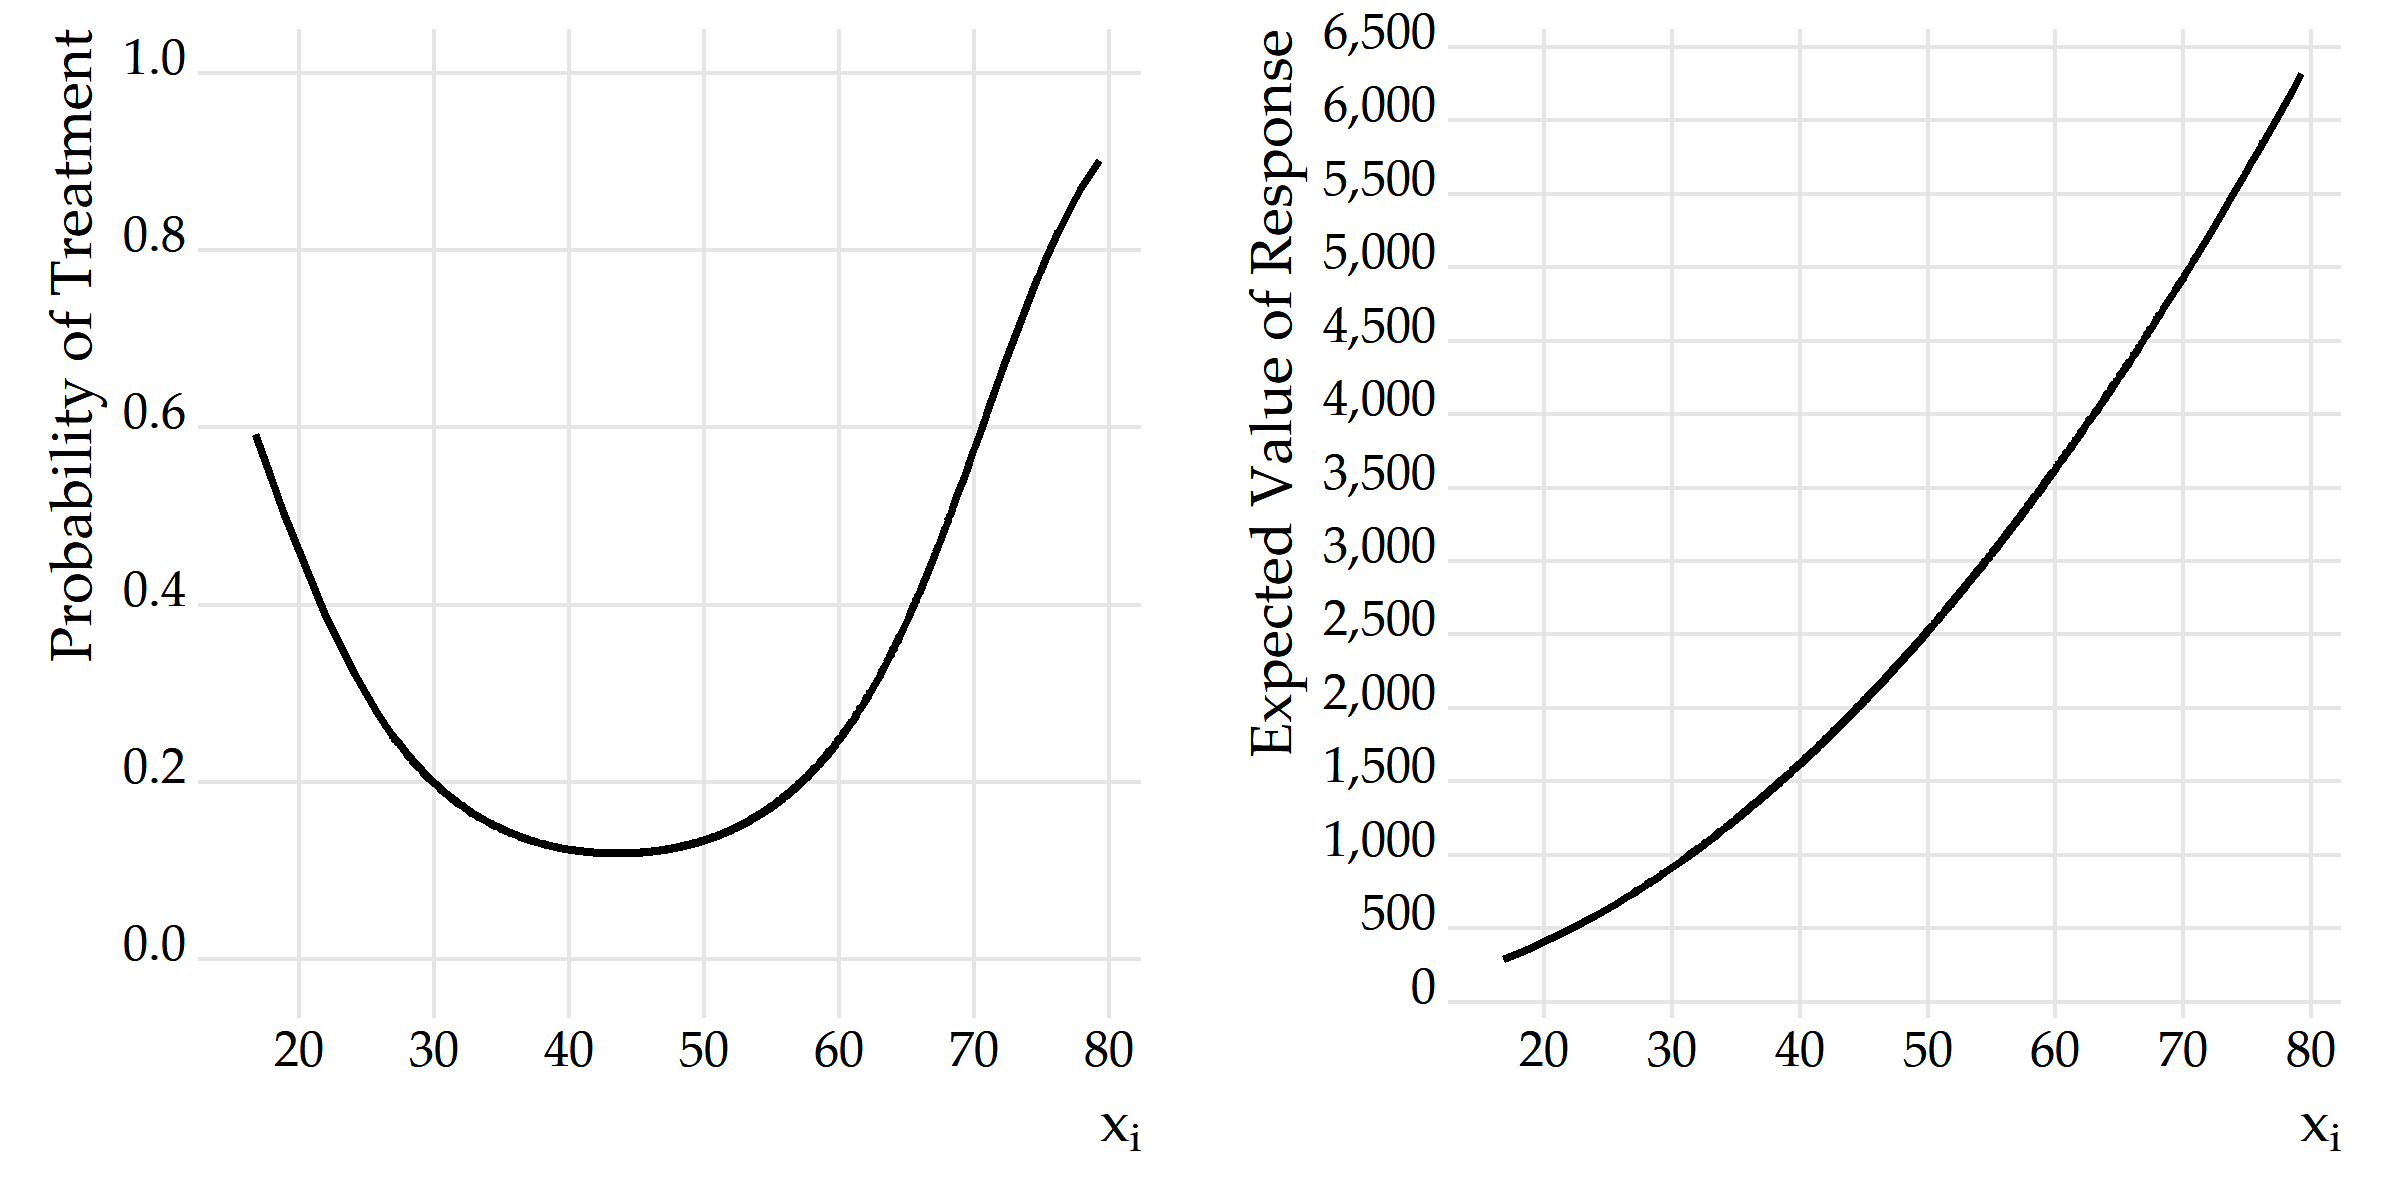
\includegraphics{treatment.png}
\caption{The nonlinear confounding influence of \(x_i\) on treatment
assigment and the conditional mean of the response.}
\end{figure}

Additionally, to demonstrate the robustness of RFA to complex functional
forms, propensity to receive treatment and values of the response are a
nonlinear function of \(x_i\). Figure 1 depicts the relationship between
\(x_i\) and probability of treatment and the conditional mean of the
response. As the figure shows, the probability that \(i\) receives
treatment is a convex curvilinear function of \(x_i\). Further, the
conditional mean of the response variable \(y_i\) is an exponential
function of \(x_i\).

\hypertarget{analysis}{%
\subsection{Analysis}\label{analysis}}

With the details of the simulated d.g.p. summarized, I now turn to the
methods I apply to recover and evaluate estimates of \(\beta\). To keep
comparisons simple, I apply three approaches to obtaining \(\beta\)
estimates: multiple regression-based adjustment, matching, and RFA.

For regression-based adjustment, I estimate the following linear model
via OLS:
\[y_i = \alpha + \beta z_i + \gamma_1 x_i + \gamma_2[z_i\cdot(x_i - \bar{x})] + \epsilon_i.\]
This interactive specification is recommended by Lin (2013). The
\(\hat{\beta}\) provided by the above represents the ATE for the average
observation and serves as a more robust estimate of the ATE than simply
additively controlling for covariates.

For matching, I rely on optimal full matching on \(x_i\) based on
Mahalanobis distance. The benefit of full matching is that it makes use
of as many observations as possible in identifying treatment and control
comparisons (Hansen and Klopfer 2006), while it also is optimal in
producing similarly matched sets of observations (Rosenbaum 1991). To
obtain an estimate of the ATE, I calculate the within matched set
difference between treatment and control observations.

Finally, I calculate causal estimates with RFA, using \(x_i\) to
residualize both \(y_i\) and \(z_i\) with random forest regression.

To make comparisons between these three approaches, I focus on four key
metrics: (1) average bias, (2) mean squared error (MSE), (3) efficiency,
and (4) overlap between nominal and effective samples. The first is
simply estimated as
\[\text{Bias}_m = \sum_{1=k}^K\frac{\hat{\beta}^m_k - \beta_\text{true}}{K},\]
for \(k = 1,...,K\) Monte Carlo replicates for a given method \(m\). The
MSE of the estimate, further, is estimated as
\[\text{MSE}_m = \sum_{1=k}^K\frac{\left(\hat{\beta}^m_k - \beta_\text{true}\right)^2}{K}.\]
Efficiency is measured as the proportion of Monte Carlo iterations that
the true ATE falls within the 95 percent confidence interval of the
estimated ATE. Estimates of parameter variance are generated with a
heteroskedasticity consistent variance-covariance matrix.

To assess the extent to which parameter estimates are generated from an
effective sample that generalizes to the nominal sample, I also estimate
the percent overlap between the effective sample distribution, and
nominal sample distribution, of \(x_i\). Following Aronow and Samii
(2016), I recover the observation specific weights produced by each of
the three measures by taking the square of the observation specific
residual variation in \(z_i\) after applying each of the adjustment
strategies. For multiple regression, this is equal to
\[w_i^\text{LR} = (z_i - \hat{z}_i)^2 \quad \text{s.t.} \quad \hat{z}_i = \hat{\eta}_0 + \hat{\eta}_1x_i + \hat{\eta}_2[z_i\cdot(x_i - \bar{x})].\]
For matching, where \(M\) is a matrix of matched set specific indicator
variables, observation weights are given as
\[w_i^M = (z_i - \hat{z}_i)^2 \quad \text{s.t.} \quad \hat{z}_i = \mathbf{M}\hat{\mu}.\]
Finally, RFA weights are estimated as
\[w_i^\text{RFA} = (z_i - \hat{z}_i)^2 \quad \text{s.t.} \quad \hat{z}_i = \hat{f}(x_i), \]
where \(\hat{f}(x_i)\) denotes the OOB of random forest predictions of
the conditional mean of \(z_i\) given \(x_i\).

With these weights, I generate two comparison distributions and
calculate the percent overlap between the two. The first distribution is
simply the unweighted distribution of \(x_i\)---this is the nominal
distribution. I then compare this to that of the effective sample
generated by each of the methods---that is, the distribution of
\(w_i^mx_i\). With these two distributions, I estimate the overlapping
coefficient, or the proportion of observations that fall within both the
nominal and effective samples. This is given as
\[\text{OVL}_m = \sum_{d=1}^D \min\{\kappa(x_i)_d,\kappa(w_i^mx_i)_d\}\]
where \(\kappa(\cdot)\) is the gaussian Kernel density estimator and
\(d\) denotes the \(d^\text{th}\) bin for \(d = 1,...,D\) bins given a
predetermined bandwidth.

\hypertarget{results}{%
\subsection{Results}\label{results}}

\hypertarget{performance-of-causal-estimates}{%
\subsubsection{Performance of Causal
Estimates}\label{performance-of-causal-estimates}}

Results are shown for \(K = 500\) simulated iterations of the d.g.p.
Table 1 shows the estimated bias, MSE, and coverage for multiple
regression, optimal full matching, and RFA. The results are shown from
best to worst in performance based on average bias.

\begin{table}[t] \centering 
  \caption{Performance of Adjustment Strategies} 
  \label{} 
\begin{tabular}{@{\extracolsep{5pt}} cccc} 
\\[-1.8ex]\hline 
\hline \\[-1.8ex] 
model & Bias & MSE & Coverage \\ 
\hline \\[-1.8ex] 
RFA & 1.415 & 14.302 & 0.968 \\ 
Matching & 6.099 & 68.619 & 1 \\ 
Multiple Regression & 62.663 & 4,685.994 & 0.344 \\ 
\hline \\[-1.8ex] 
\end{tabular} 
\end{table}

RFA performs the best, followed by matching and multiple regression. The
RFA generated estimate of the ATE displays only a slight upward bias, on
average returning a \(\hat{\beta}\) 1.42 units higher than the true ATE.
The MSE for RFA was further 14.3, and its 95 percent CI contained the
true ATE 96.8 percent of the time.

Matching, meanwhile, returned an estimate of the ATE that was, on
average, 6.1 units greater than the true ATE of 5. Further, the MSE for
matching was 69.62 and coverage was 100 percent, suggesting wider than
expected variance in the ATE estimates.

Finally, multiple regression returned an estimate of the ATE that was,
on average, several magnitudes larger than the true ATE---62.66 units
greater than the true ATE of 5. The MSE, further, was a staggering
4,685.99. In addition, coverage was only about 34.4 percent, which is
far less that what we would expect for 95 percent CIs.

Figure 2 shows the distribution of ATE estimates from the simulation.
The results show that RFA estimates most closely center around the true
ATE, while matching comes in at a close second. Meanwhile, the
distribution of estimates recovered by multiple regression barely
overlap with the true ATE.

\begin{figure}
\centering
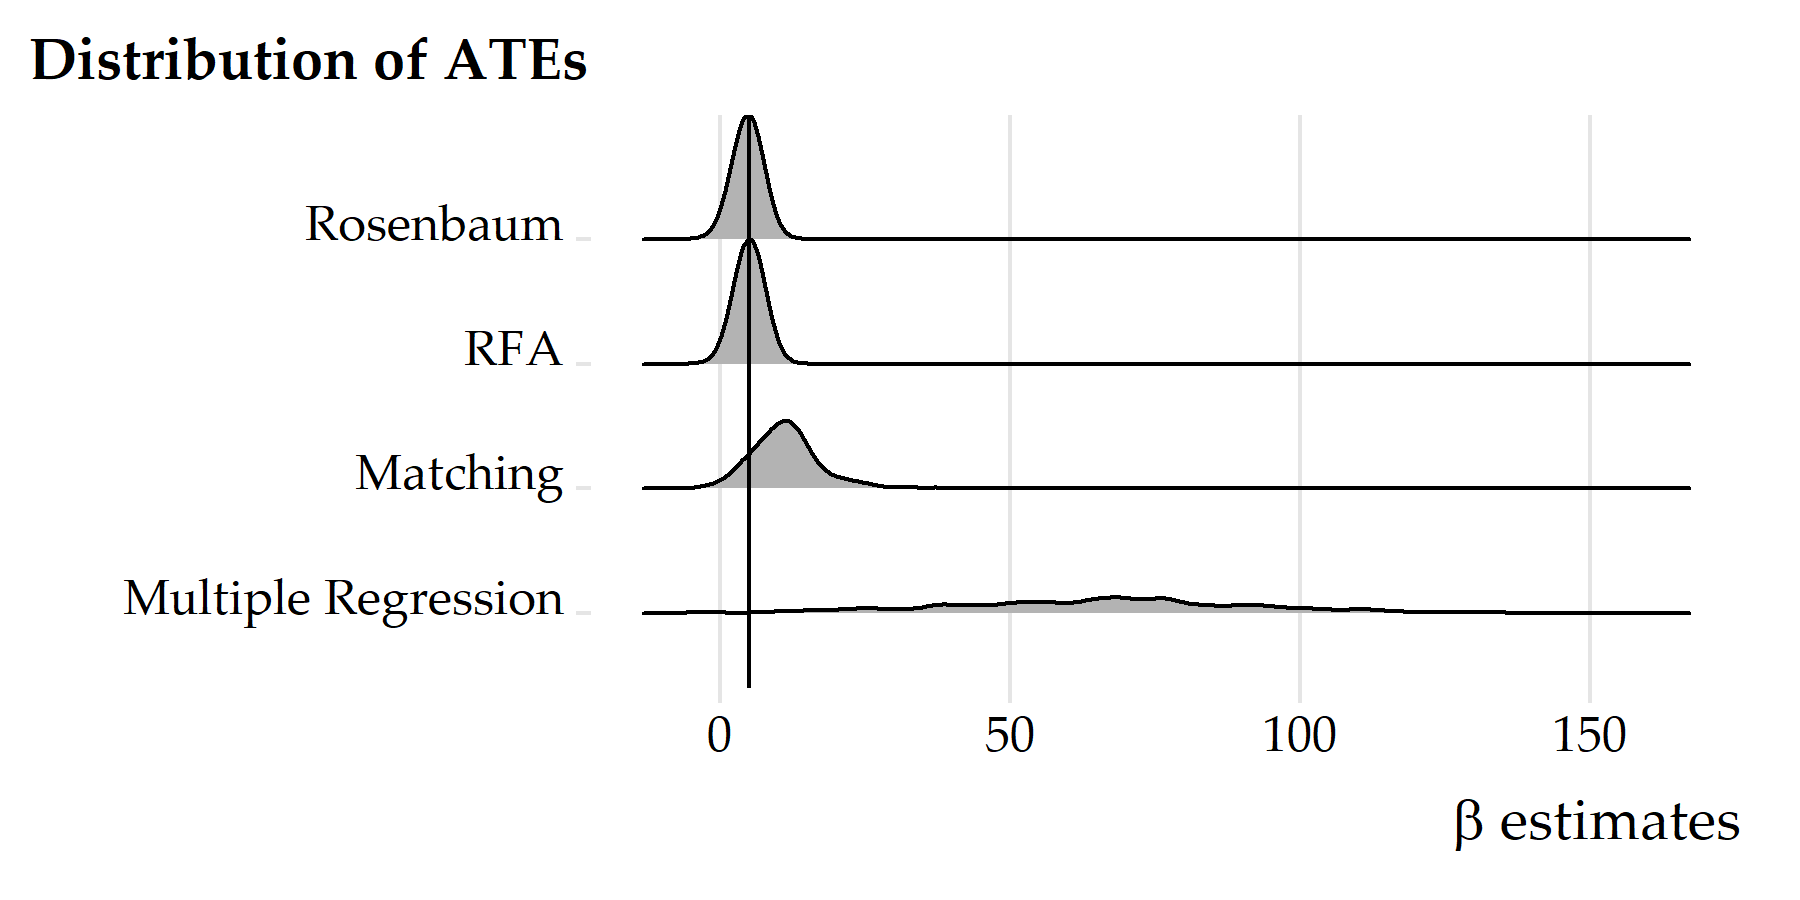
\includegraphics{ate_distributions.png}
\caption{Variation in ATE estimates recovered by multiple regression,
optimal full matching, and RFA. Results from 500 simulated iterations.
The black vertical line denotes the value of the true ATE.}
\end{figure}

\hypertarget{nominal-vs.-effective-samples}{%
\subsubsection{Nominal vs.~Effective
Samples}\label{nominal-vs.-effective-samples}}

The foregoing results highlight the robustness of RFA. However, at best,
they merely demonstrate that RFA scores high on internal validity. How
well do RFA estimates generalize?

The results shown in Figure 3 offer an answer to this question. Shown
are the distributions of overlapping coefficients for each of the
simulated iterations. The greater the overlap, the greater the
percentage of observations that fall both within the nominal and
effective samples.

\begin{figure}
\centering
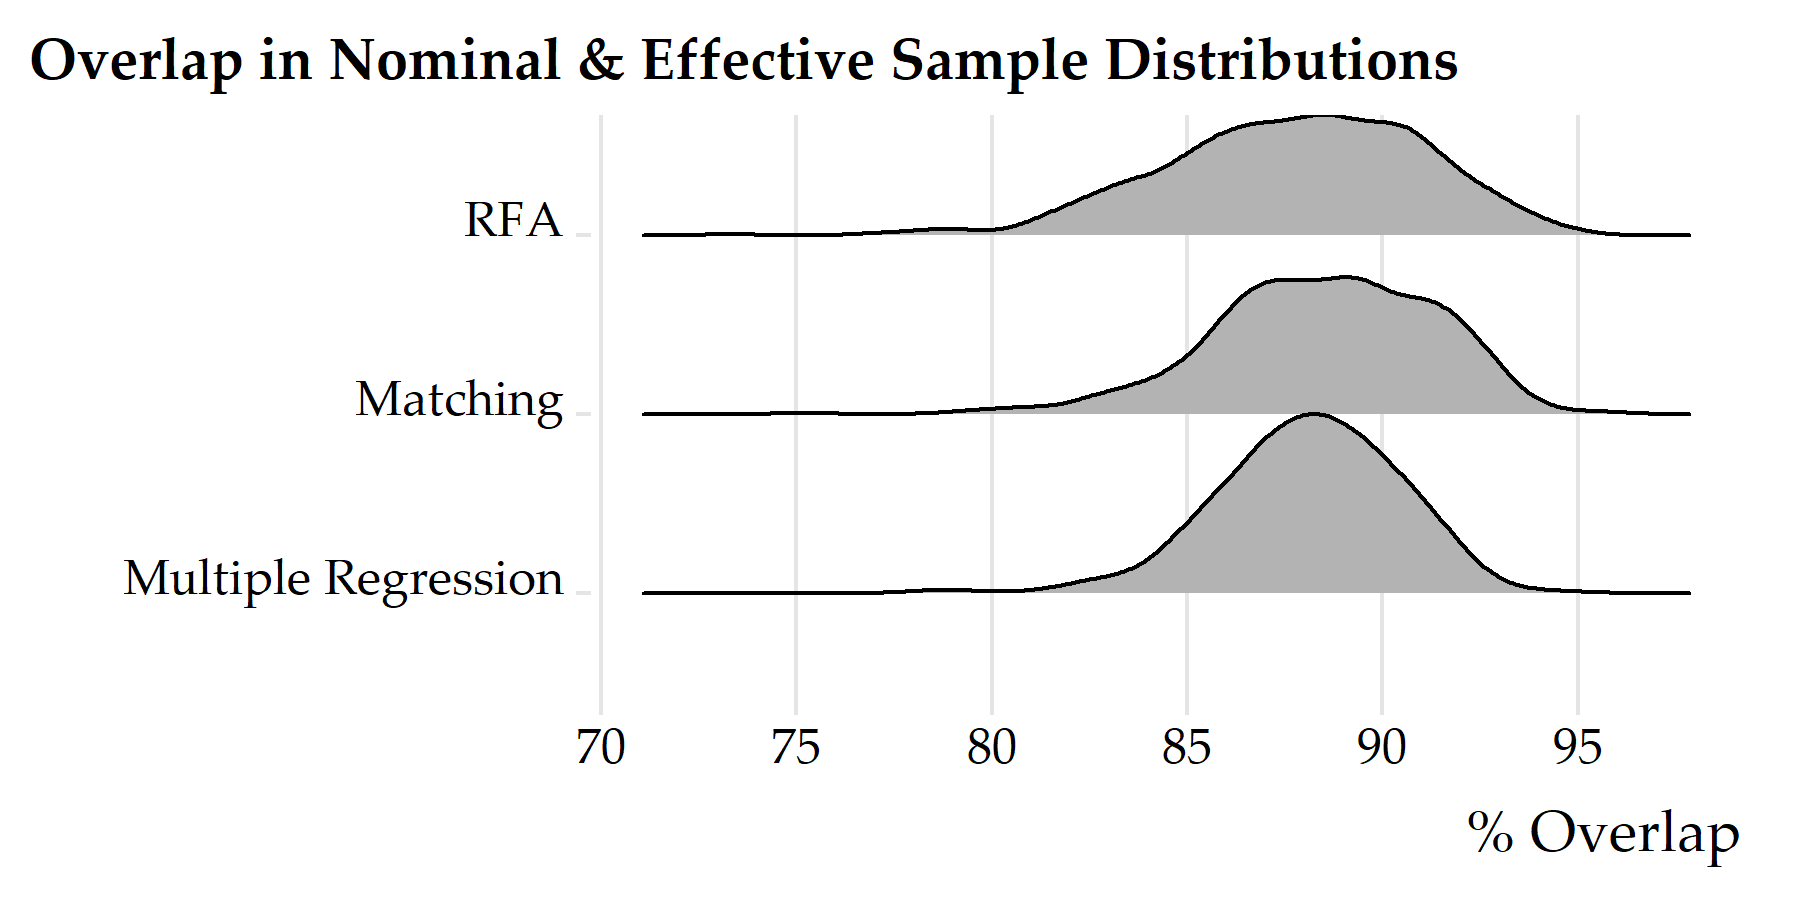
\includegraphics{overlap_distribution.png}
\caption{The percentage overlap between nominal and effective samples
for each method across Monte Carlo replicates.}
\end{figure}

In settings with nonrandom treatment assignment, 100 percent overlap is
rarely possible. The idea that using multiple regression or matching
with a large, observational dataset ensures greater external validity is
a common fallacy---albeit, an understandable one. However, the effective
sample that such methods use to actual estimate a causal effect often
differs substantially from the nominal sample.

This much is apparent for each of the methods considered here---even for
RFA. However, if external validity is a concern, RFA may be the optimal
choice. In comparing the distribution of overlapping coefficients per
each simulated iteration, the effective sample used by RFA has nearly
double the overlap with the nominal sample relative to matching and
multiple regression. On average, the effective samples from multiple
regression and matching overlap with the nominal sample 10 and 12.6
percent of the time. The effective sample from RFA, meanwhile, overlaps
with the nominal sample, on average, 22.1 percent of the time. This is
an appreciable and statistically significant improvement in the degree
to which the effective sample generalizes to the nominal.

\hypertarget{application-to-real-world-data}{%
\section{Application to Real-World
Data}\label{application-to-real-world-data}}

To demonstrate the application of RFA, I replicate analysis done by
Nielsen et al.~(2011). The authors test the effect of so-called ``aid
shocks'' on the probability of civil war in countries that receive
Official Development Assistance (ODA). An aid shock is defined as a
sudden change in total aid received as a proportion of gross domestic
product (GDP). The authors code a decline in aid per GDP at or below the
15\(^\text{th}\) percentile for the entire sample of cases in their
analysis as a \emph{negative} aid shock, and an increase in aid per GDP
at or above the 85\(^\text{th}\) percentile as a \emph{positive} aid
shock.

Shocks in aid flows are theorized to influence the likelihood of armed
conflict between a government and potential insurgents via a number of
pathways. One is that governments may use aid to supplement
side-payments to opposing factions. By ``buying off'' potential
insurgents, states hope to reduce the likelihood of conflict.

A second pathway is the impact of aid flows on power parity between the
state and insurgents. A sudden decline in ODA is presumed to improve the
power of insurgents relative to the state due to loss of aid revenue.
Consequently, the state is left with fewer resources, improving rebels'
perceived chances of victory in armed conflict.

The authors hypothesize that negative aid shocks increase the
probability of conflict. However, they offer reasons to expect either a
positive or negative effect of positive aid shocks. A negative effect
follows from logic that mirrors that give above: more aid means more
resources for the state to use as side payments and to combat
insurgents. Conversely, windfalls in aid may incite bargaining problems
between the government and opposition groups. With an increase in
resources comes conflict over how those resources should be distributed,
and insurgents may demand more that they previously were receiving. The
authors, therefore, leave the question of the effect of positive aid
shocks to empirical investigation.

In their analysis, Nielsen et al.~(2011) find that negative aid shocks
increase the probability of armed conflict. Meanwhile, positive aid
shocks have a null effect---perhaps as a result of the cross-cutting
forces highlighted above. For their analysis, the authors use both
regression-based adjustment (via logistic regression) and genetic
matching to generate these findings. Here, I apply RFA to this question,
alongside the two approaches I used in the previous simulation---optimal
full matching and multiple regression.

\hypertarget{the-data}{%
\subsection{The Data}\label{the-data}}

With the replication dataset made available by Nielsen et al.~(2011), I
estimate the effect of \emph{aid shocks} on the incidence of \emph{civil
war}. After multiple imputation with random forests, the sample includes
201 aid recipient countries from 1975 to 2007 for a total of 5,130
country-year observations.

Following the authors, I control for the following confounding
variables: human rights violations, number of assassinations, number of
riots, number of strikes, number of anti-government demonstrations,
infant mortality, number of contiguous countries experiencing a civil
war, regime type, poverty, population, ethnic and religious
fractionalization, the Cold War, mountainous terrain, noncontiguousness,
and year. All time-varying variables are lagged by one year.

The authors, in their main specification, code an aid shock as occurring
when the change in aid per GDP is less than or equal to the
15\(^\text{th}\) percentile for the entire sample. Because this
threshold is arbitrary, and since the estimated effect of an aid shock
may be sensitive to the cutoff used, I calculate the effect of aid
shocks across a range of percentile cutoffs (the 15 to the 85
percentiles in increments of 10). For all shocks coded below the
50\(^\text{th}\) percentile, I code the shock as negative (all values
less than or equal to the cutoff are coded as 1). Conversely, for all
shocks above the 50\(^\text{th}\) percentile, I code the shock as
positive (all values greater than or equal to the cutoff are coded as
1). Varying the cutoff in this way allows me to observe the validity of
different aid shock thresholds and to see whether negative shocks have
differential effects from positive shocks.

\begin{figure}
\centering
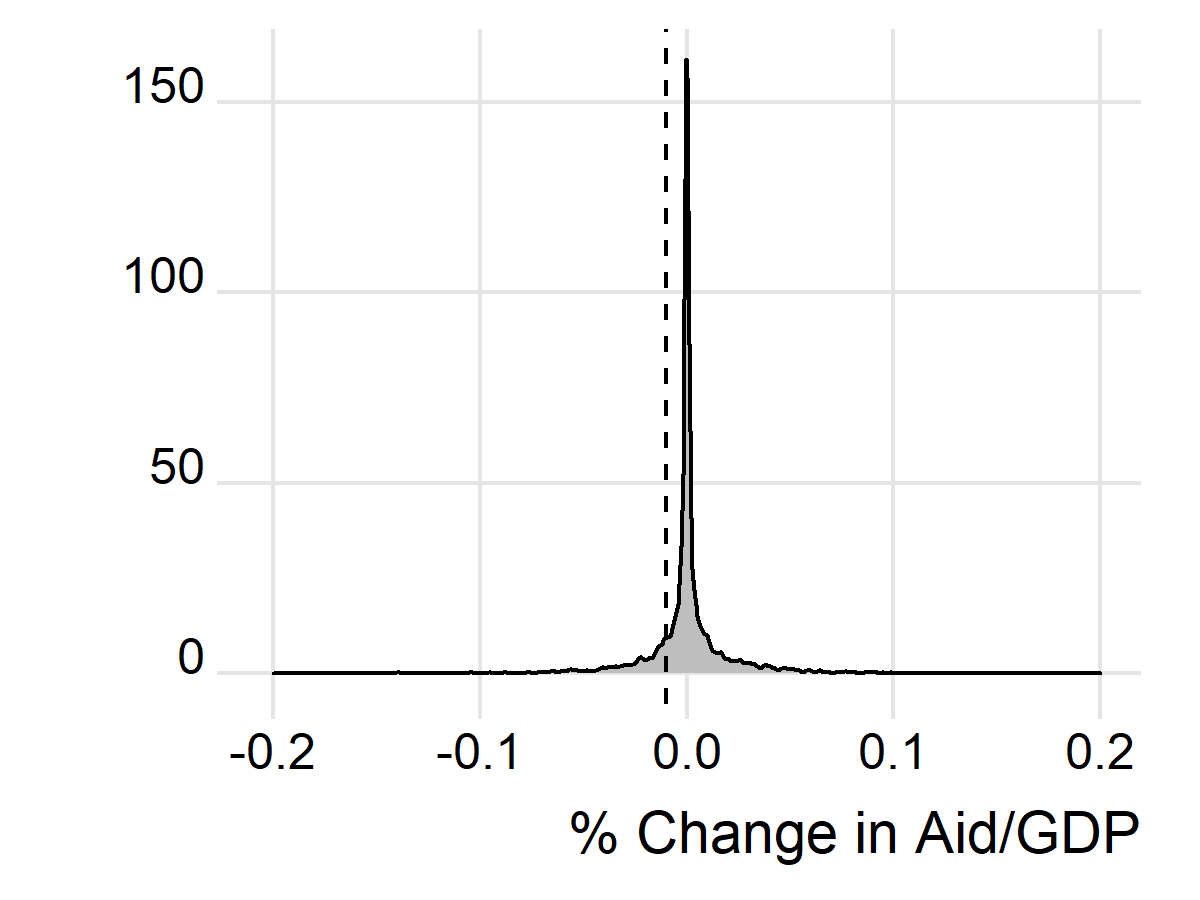
\includegraphics{histplot.png}
\caption{Distribution of the causal variable (percent change in
aid/GDP). The vertical line denotes the 15th percentile.}
\end{figure}

Figure 4 shows the distribution of values of percent change in total aid
received by states per GDP. The dashed vertical line denotes the
15\(\text{th}\) percentile. Inexplicably, this value differs from that
calculated by Nielsen et al.~Nevertheless, since I use different
percentile cutoffs in the analysis, the difference between the value
identified as the cutoff point for aid shocks by the authors and my own
is not of much concern.

\hypertarget{analysis-1}{%
\subsection{Analysis}\label{analysis-1}}

To recover estimates of the effect of aid shocks on civil war onset, I
use the same three approaches as in the previous simulation. In addition
to RFA, I use optimal full matching, as well as regression-based
adjustment.\footnote{For matching, I use the `fullmatch` function in the `optmatch` package in `R`.}

\begin{figure}
\centering
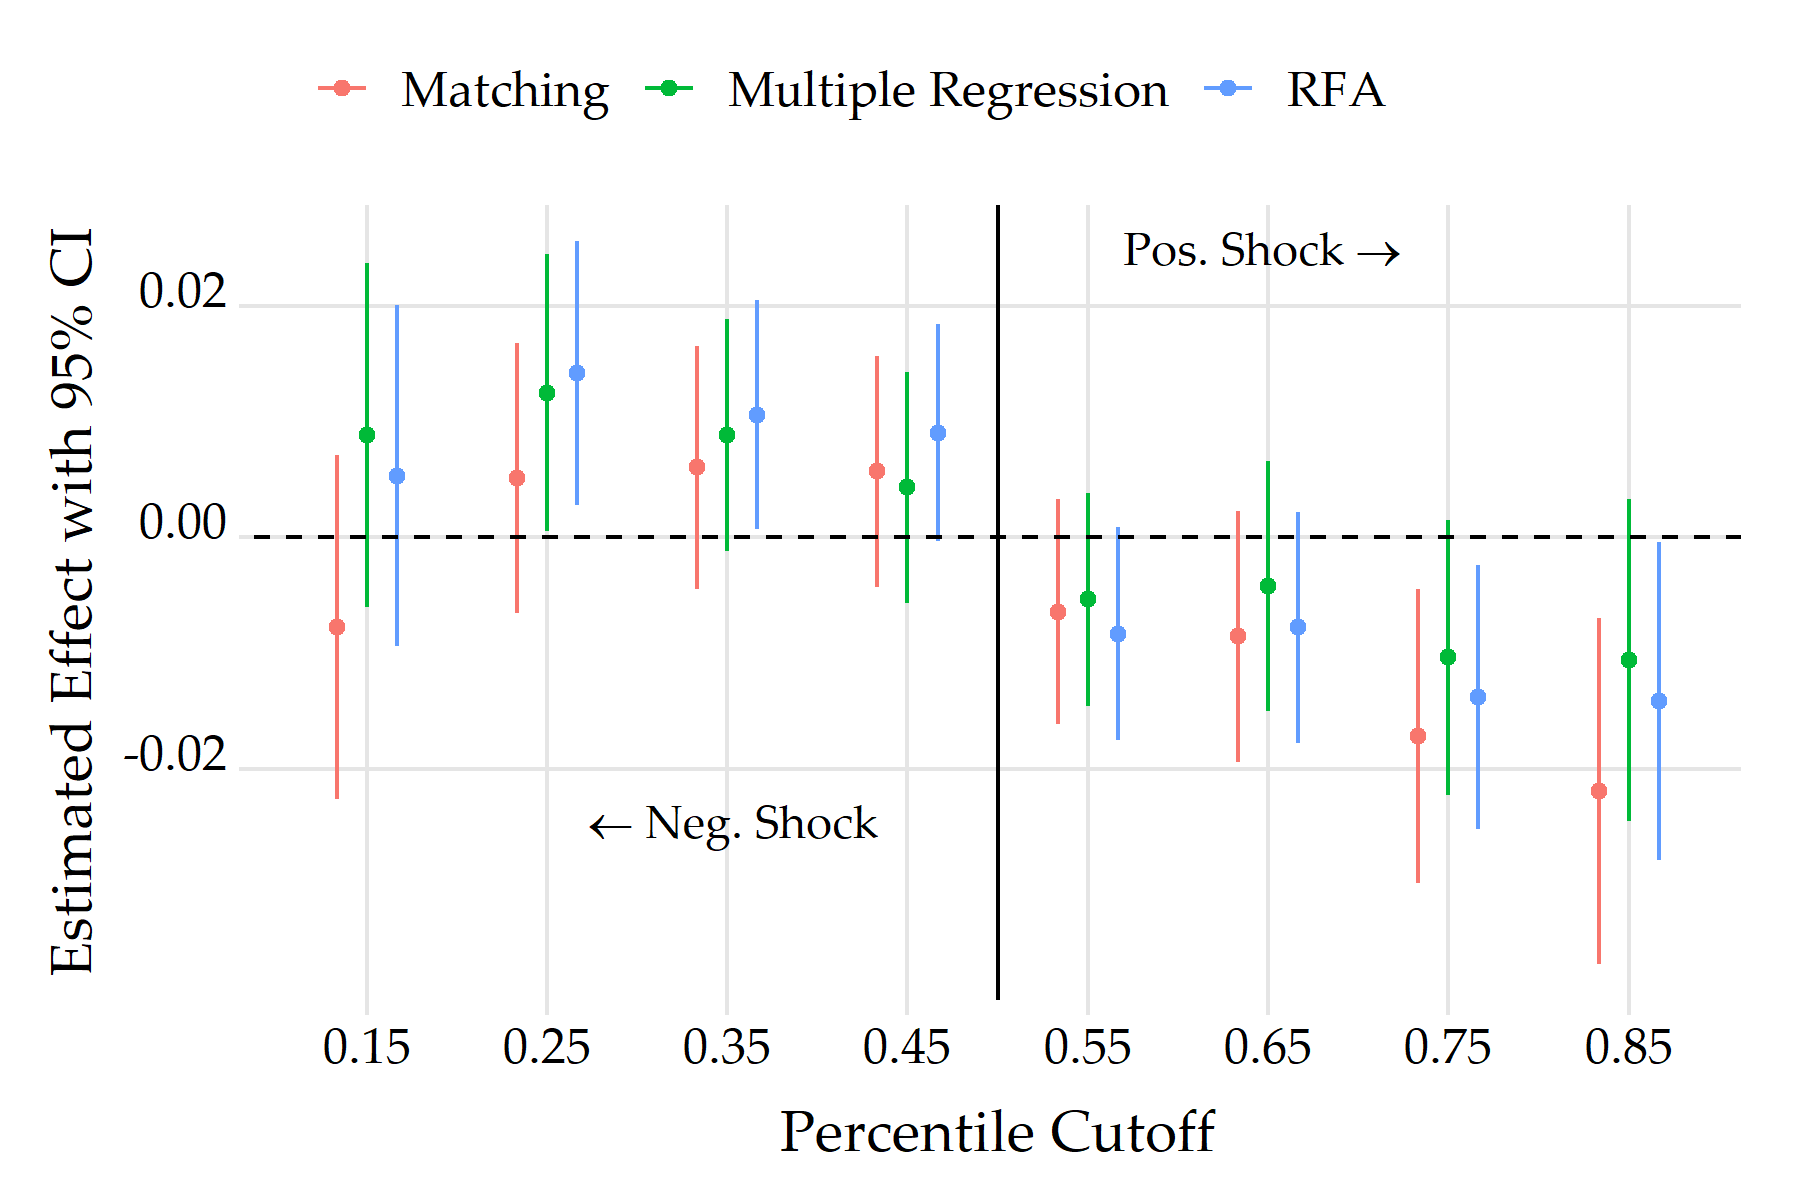
\includegraphics{allcoef.png}
\caption{The effect of aid shocks on the probability of civil war. Blue
estimates obtained via RFA. Red estimates obtained via optimal full
matching. Green estimates obtained via multiple regression. 95 percent
CIs calculated from robust standard errors. Results shown with different
cutpoints for ``aid shocks.''}
\end{figure}

Figure 5 shows RFA, genetic matching, and OLS estimates of the effect of
aid shocks on the probability of civil war onset. Results are shown for
varying cutoff points for aid shocks. Unlike Nielsen et al.~(2011), I am
unable to recover evidence of a significant effect of aid shocks at the
15\(\text{th}\) percentile, regardless of method used. More puzzling,
the estimate returned by matching is negative, suggesting a marginal
decline in the probability of civil war. However, at the 25\(\text{th}\)
percentile, both RFA and multiple regression return a significant and
positive estimate of the effect of a negative shock in aid flows on the
likelihood of civil war. Further, while not statistically significant,
matching as well returns a positive estimate.

In terms of positive aid shocks, only RFA and matching return a
significant and negative estimate for the probability of civil war, and
only for increases in aid at or greater than the 75\(\text{th}\)
percentile---contrary to the findings of Nielsen et al.~(2011) who fail
to identify a significant effect for positive aid shocks.

\begin{figure}
\centering
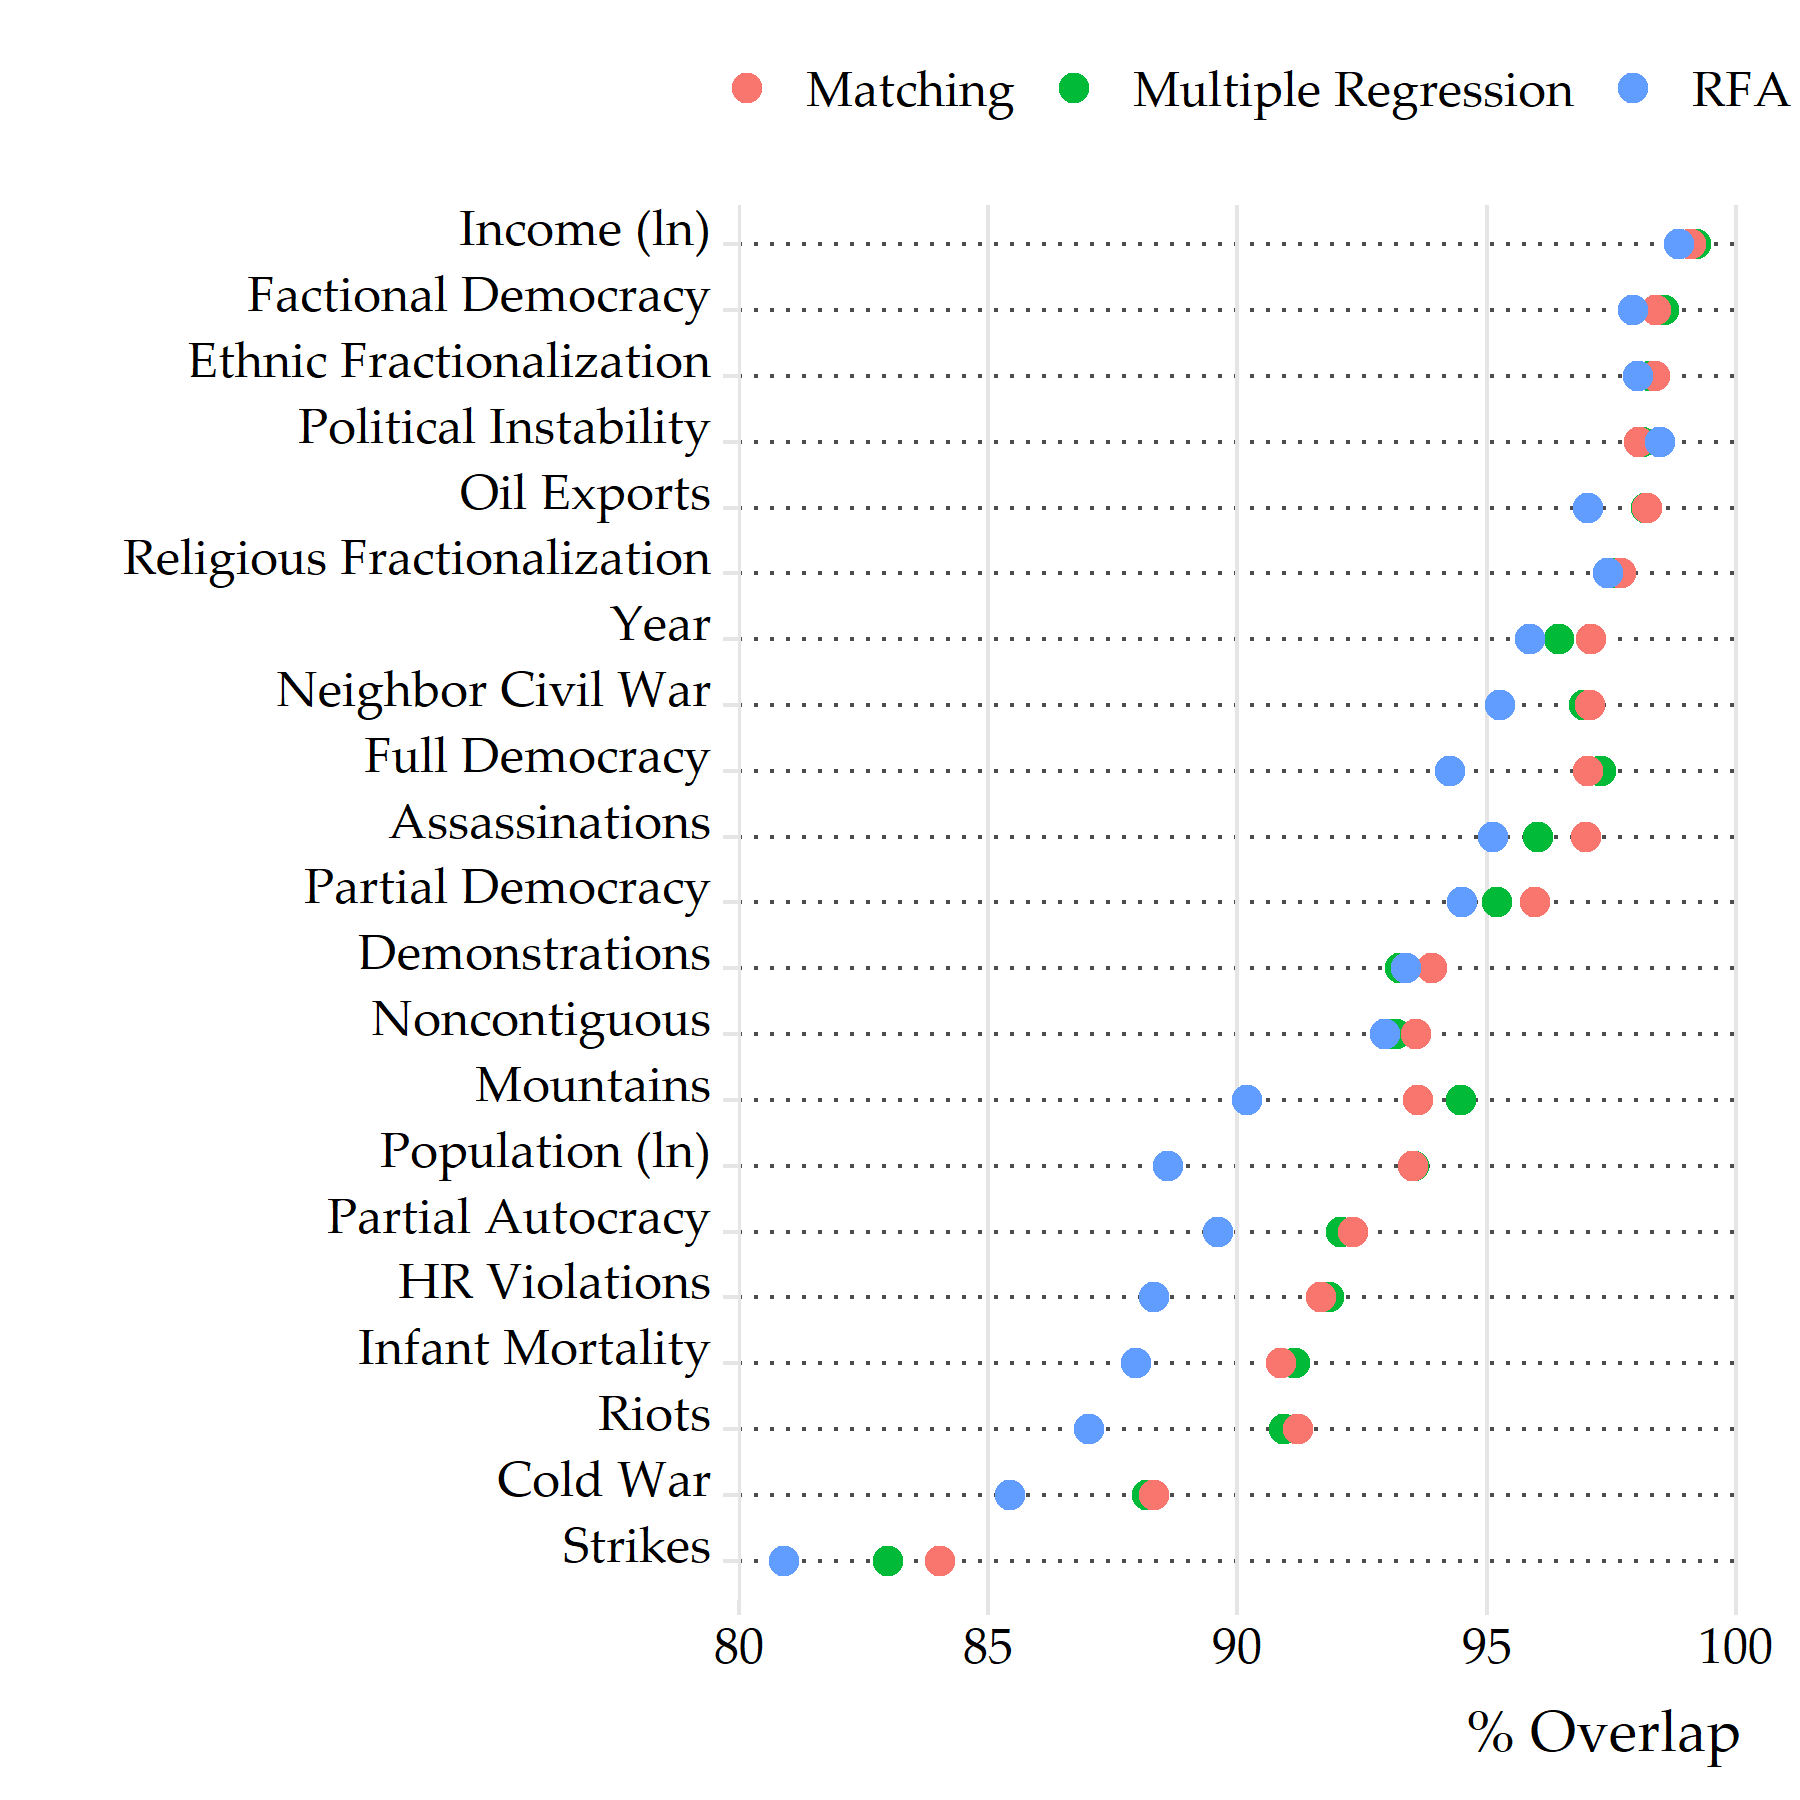
\includegraphics{overlap_civilwar.png}
\caption{The degree of overlap between the nominal and effective samples
for RFA, matching, and multiple regression.}
\end{figure}

\begin{table}[t] \centering 
  \caption{Best Coverage across Covariates} 
  \label{} 
\begin{tabular}{@{\extracolsep{5pt}} lc} 
\\[-1.8ex]\hline 
\hline \\[-1.8ex] 
 & Best Coverage for $N$ Covariates \\ 
\hline \\[-1.8ex] 
Matching & 3 \\ 
Multiple Regression & 6 \\ 
RFA & 12 \\ 
\hline \\[-1.8ex] 
\end{tabular} 
\end{table}

To assess the degree to which estimates returned by RFA, matching, and
multiple regression generalize to the nominal sample of cases, I
calculated the overlapping coefficient per each confounding covariate
per each method. I used negative aid shocks at the 15\(\text{th}\)
percentile as the treatment variable in calculating overlap. Estimates
are shown in Figure 6. The degree of overlap between effective and
nominal samples differs markedly across covariates. While some have
nearly 50 percent overlap (infant mortality, the Cold War dummy,
religious fractionalization, income, and political instability), one has
next to zero (oil exports). Overlapping coefficients further appear
correlated across estimators, suggesting that each of the methods
estimates the ATE of aid shocks using roughly similar effective samples.

However, despite marginal similarities in overlap, RFA has a noticeable
edge. Table 2 shows the number of covariates for which each method's
overlapping coefficient is greatest. Matching only displays greatest
overlap for 3 of the 21 covariates. Multiple Regression does slightly
better with greatest overlap for 6 covariates. RFA, however, has the
greatest overlapping coefficients for 12 of the 21 covariates---twice
that of multiple regression, and four times that of matching. Though it
is important to avoid making too much of these differences---imperfect
and limited overlap is to be expected, not to mention necessary, for
recovering estimates based on appropriate comparisons in the data---RFA
nonetheless bases estimates on a slightly more representative sample, as
it did in the previous simulation.

\begin{table}[!htbp] \centering 
  \caption{Difference between Effective and Nominal Samples} 
  \label{} 
\begin{tabular}{@{\extracolsep{5pt}} ccccc} 
\\[-1.8ex]\hline 
\hline \\[-1.8ex] 
 & variable & Regression & Matching & RFA \\ 
\hline \\[-1.8ex] 
1 & HR Violations & 0.11\textasteriskcentered \textasteriskcentered \textasteriskcentered  & 0.11\textasteriskcentered \textasteriskcentered \textasteriskcentered  & 0.14\textasteriskcentered \textasteriskcentered \textasteriskcentered  \\ 
2 & Assassinations & 0.02\textasteriskcentered \textasteriskcentered \textasteriskcentered  & 0.02\textasteriskcentered \textasteriskcentered \textasteriskcentered  & 0.02\textasteriskcentered \textasteriskcentered \textasteriskcentered  \\ 
3 & Riots & -0.1\textasteriskcentered \textasteriskcentered \textasteriskcentered  & -0.09\textasteriskcentered \textasteriskcentered \textasteriskcentered  & -0.11\textasteriskcentered \textasteriskcentered \textasteriskcentered  \\ 
4 & Strikes & -0.4\textasteriskcentered \textasteriskcentered \textasteriskcentered  & -0.37\textasteriskcentered \textasteriskcentered \textasteriskcentered  & -0.44\textasteriskcentered \textasteriskcentered \textasteriskcentered  \\ 
5 & Demonstrations & -0.27\textasteriskcentered \textasteriskcentered \textasteriskcentered  & -0.18\textasteriskcentered \textasteriskcentered \textasteriskcentered  & -0.15\textasteriskcentered \textasteriskcentered \textasteriskcentered  \\ 
6 & Infant Mortality & -2.4\textasteriskcentered \textasteriskcentered \textasteriskcentered  & -2.09\textasteriskcentered \textasteriskcentered \textasteriskcentered  & -2.55\textasteriskcentered \textasteriskcentered \textasteriskcentered  \\ 
7 & Neighbor Civil War & 0.03\textasteriskcentered \textasteriskcentered \textasteriskcentered  & 0.03\textasteriskcentered \textasteriskcentered \textasteriskcentered  & 0.04\textasteriskcentered \textasteriskcentered \textasteriskcentered  \\ 
8 & Partial Autocracy & 0.05\textasteriskcentered \textasteriskcentered \textasteriskcentered  & 0.05\textasteriskcentered \textasteriskcentered \textasteriskcentered  & 0.06\textasteriskcentered \textasteriskcentered \textasteriskcentered  \\ 
9 & Partial Democracy & 0.01\textasteriskcentered \textasteriskcentered  & 0.01\textasteriskcentered \textasteriskcentered \textasteriskcentered  & 0.01\textasteriskcentered \textasteriskcentered \textasteriskcentered  \\ 
10 & Factional Democracy & -0.01. & -0.02. & -0.02\textasteriskcentered \textasteriskcentered  \\ 
11 & Full Democracy & -0.01  & 0  & 0  \\ 
12 & Income (ln) & 0  & 0.01  & 0.01  \\ 
13 & Population (ln) & -0.06\textasteriskcentered \textasteriskcentered \textasteriskcentered  & -0.05\textasteriskcentered \textasteriskcentered \textasteriskcentered  & -0.07\textasteriskcentered \textasteriskcentered \textasteriskcentered  \\ 
14 & Oil Exports & 0.23  & 0.24  & 0.3\textasteriskcentered  \\ 
15 & Political Instability & 0  & 0.02  & -0.02. \\ 
16 & Ethnic Fractionalization & 0  & 0.01. & 0.01  \\ 
17 & Religious Fractionalization & -0.03  & 0  & -0.05\textasteriskcentered \textasteriskcentered  \\ 
18 & Cold War & 11.46\textasteriskcentered \textasteriskcentered \textasteriskcentered  & 11\textasteriskcentered \textasteriskcentered \textasteriskcentered  & 14.08\textasteriskcentered \textasteriskcentered \textasteriskcentered  \\ 
19 & Mountains & 0.08\textasteriskcentered \textasteriskcentered \textasteriskcentered  & 0.09\textasteriskcentered \textasteriskcentered \textasteriskcentered  & 0.1\textasteriskcentered \textasteriskcentered \textasteriskcentered  \\ 
20 & Noncontiguous & 0.05\textasteriskcentered \textasteriskcentered \textasteriskcentered  & 0.04\textasteriskcentered \textasteriskcentered \textasteriskcentered  & 0.06\textasteriskcentered \textasteriskcentered \textasteriskcentered  \\ 
21 & Year & 0.03\textasteriskcentered \textasteriskcentered \textasteriskcentered  & 0.03\textasteriskcentered \textasteriskcentered \textasteriskcentered  & 0.04\textasteriskcentered \textasteriskcentered \textasteriskcentered  \\ 
\hline \\[-1.8ex] 
\end{tabular} 
\end{table}





\newpage
\singlespacing 
\end{document}